\documentclass[a4paper,11pt]{report}
\usepackage[portuguese]{babel}

% * conseguir manusear uma variedade de símbolos usados nos diferentes grupos de línguas
\usepackage[latin1,utf8]{inputenc}

% * colorir textos
\usepackage{graphicx}
% * capa com imagem
\usepackage{titlepic}

% * tamanho das margens
\usepackage{geometry}

% * multiplas colunas
\usepackage{multicol}

% * referencias dentro do ficheiro
\usepackage{hyperref}
\usepackage{xurl}  % * Quebra a url de forma inteligente

\usepackage{booktabs, multirow} % * Para bordas das tabelas
\usepackage{soul}% * Para o sublinhado
\usepackage{xcolor,colortbl} % * Cores nas células
\usepackage{changepage,threeparttable} % * Tabelas largas.


% *O Documento tem de ter margens superior e inferior de 1.5 cm e margens
% *   esquerda e direita de 1 cm;
\geometry{a4paper, left= 1 cm, right= 1 cm, top= 1.5 cm, bottom= 1.5 cm }

% * Titulo
\title{
		\Huge{\textbf{Finanças pessoais}} \\
		\vskip 0.25cm
		\small{Produção de Documentos Técnicos} \\
}


% * Data da entrega de trabalho
\date{24 de Novembro de 2024}

% * Nome completo
% * Número de aluno
% * Email
% * Turma que pertence
% * Nome da sua Licenciatura
\author{
	\small{ Arthur Sepulven de Aguiar } \\
	\small{ Nº de Aluno 64726 - TP 18 - fc64726@alunos.fc.ul.pt} \\
	\small{Licenciatura em Engenharia Informática} \\
}

% * Imagem relativa ao tema
\titlepic{
	% * Roxo escuro -> #6658fe
	% * Roxo Claro -> #e1ddfe
	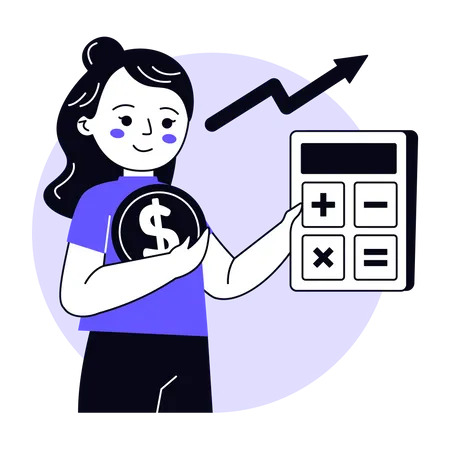
\includegraphics[width=12cm]{./first_page.jpg}
}

% \thispagestyle{empty}

\begin{document}
	% * Todos os índices (conteúdo, tabelas e figuras) são automáticos, 
	% *   feitos pelo LaTeX e estas páginas têm   paginação em numeração romana;
	\pagenumbering{Roman}
	\maketitle

	%  * Índices
	\tableofcontents % * faz o índice

	% * Depois de toda a informação que consultou, em duas colunas, diga-nos
	% * o que descobriu com esta pesquisa, se acha vantajoso fazer e manter um orçamento atualizado.
	% * um texto com o máximo de uma página sobre finanças pessoais.
	\chapter{Introdução}
		\begin{multicols}{2}

			\section{Definição \cite{intro:intro}}
				\hspace{1cm} Finanças é a ciência da administração do dinheiro. A gestão financeira pessoal é a maneira na \
				qual se controla e conhece seus gastos e lucros, uma boa gestão consiste no equilíbrio entre receitas e despesas.

			\section{Conseguência das Finanças pessoais \cite{intro:desenvolvimento}}
				\hspace{1cm} A falta de educação financeira pessoal manifesta-se tanto no nível individual quanto no social. \
				Do ponto de vista individual, decisões financeiras impactam diretamente a vida pessoal e familiar,\
				podendo contribuir para uma existência estável ou, ao contrário, gerar instabilidade. \
				Já no contexto social, tais decisões influenciam fatores como a redução da desigualdade, \
				a diminuição da pobreza intergeracional, o estímulo à inovação e ao empreendedorismo. \
				No entanto, quando mal conduzidas, essas decisões podem agravar os mesmos problemas.
			
			\section{Orçamento \cite{intro:orcamento}}
				\hspace{1cm} Criar um orçamento pessoal é um dos primeiros passos para garantir uma gestão financeira eficaz. \
				Para isso, é recomendado que você se eduque financeiramente, avalie suas receitas e despesas, estabeleça \
				metas financeiras, crie um fundo de emergência, divida seu orçamento, ajuste-o regularmente, utilize ferramentas \
				para o controle financeiro e mantenha disciplina. Um orçamento pessoal não precisa ser complexo. Com um pouco de \ 
				educação financeira, organização e disciplina, qualquer indivíduo pode criar um plano eficaz para suas finanças pessoais.

			\section{Conclusão}
				\hspace{1cm} Portanto, o planejamento das despesas e receitas pessoais é imprescindível para qualquer adulto \
				que deseje uma vida estável e sustentável. A gestão das despesas e dos custos vai para além dos efeitos no \
				indivíduo, afetando a sociedade como um todo. Um bom planejamento das finanças tem efeitos que se estendem \
				por várias gerações. Concluo que, de facto, a gestão das finanças pessoais é vantajosa.
		\end{multicols}

		\vskip 0.5cm

		\begin{multicols}{2}
			\section{Citação \cite{intro:citacao}} % * Insira também uma citação relativa ao tema.
			\vskip -1cm
			\begin{center}
				\begin{quote}
					\LARGE
					\emph{"The number one problem in today’s generation and economy is the lack of financial literacy."}
				\end{quote}
				\normalsize{O maior problema na geração e economia atual é a falta de literatura financeira.} \\
			\end{center}
			\vskip -1cm
			\begin{center}
				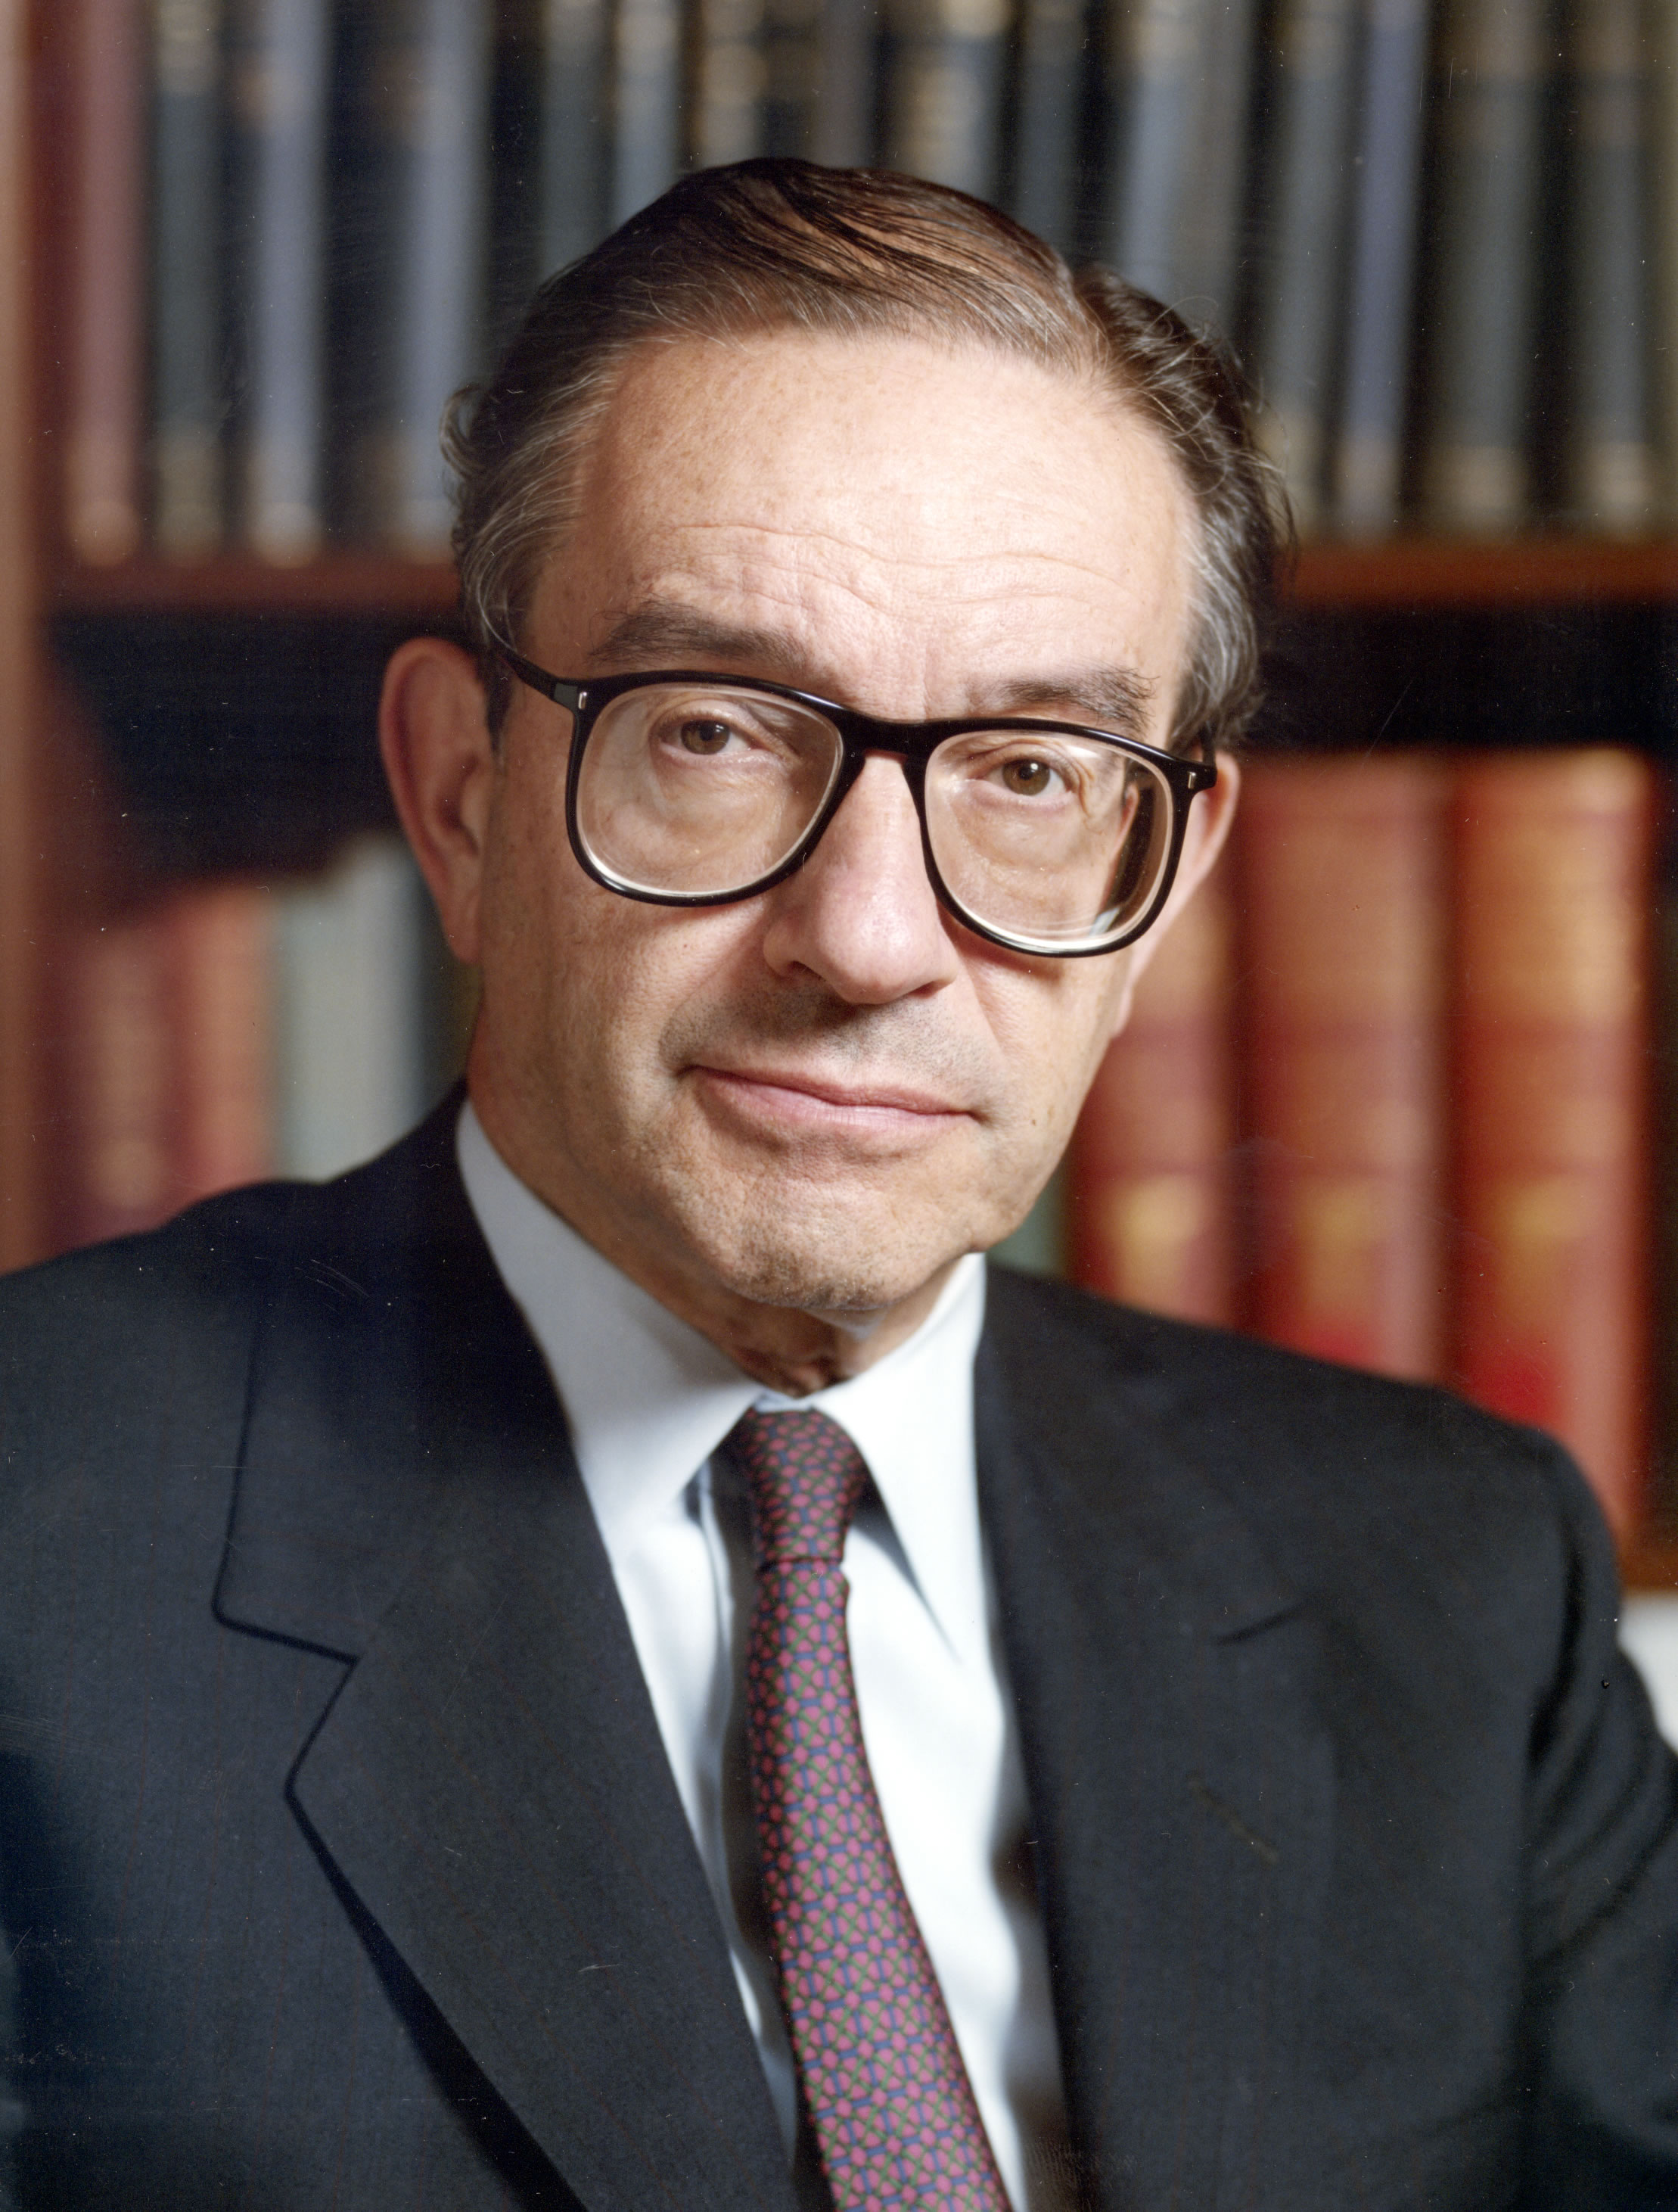
\includegraphics[width=5cm]{./alan_greenspan.jpg} \\
				\Large \textbf{- Alan Greenspan \cite{intro:bibliografia}}
			\end{center}
		\end{multicols}

		\chapter{Gestão de Finanças Pessoais}
			\begin{minipage}{\textwidth}
				\hspace{1cm} Neste caso de estudo temos um estudante universitário, com idade inferior a 23 anos \
				de idade e do sexo masculino, que possui família em uma cidade vizinha. O estudante reside em um quarto \
				compartilhado com um colega, e possui uma dieta a base de vegetais e proteínas, refeições planejadas e \
				almoça na cantina da faculdade.  Sempre possui medicamentos de reserva para pequenos problemas de saúde, 
				vai ao dentista uma vez ao ano. Possui o passe gratuito sub 23 e visita a sua família uma vez ao mês. 
			\end{minipage}

		% ** Planeamento das finanças pessoais
		% ***********************************
		\begin{table}[!htp]\centering

			\scriptsize
			\begin{tabular}{lrrrrrrrr}\toprule
				PLANEAMENTO &Setembro &Outubro &Novembro &Dezembro &Janeiro &Fevereiro &TOTAL \\\midrule
				Salário &820.00€ &820.00€ &820.00€ &820.00€ &820.00€ &820.00€ &\cellcolor[HTML]{4285f4}4,920.00€ \\
				\cellcolor[HTML]{4285f4}RENDIMENTOS &\cellcolor[HTML]{4285f4}729.80€ &\cellcolor[HTML]{4285f4}729.80€ &\cellcolor[HTML]{4285f4}729.80€ &\cellcolor[HTML]{4285f4}729.80€ &\cellcolor[HTML]{4285f4}729.80€ &\cellcolor[HTML]{4285f4}729.80€ &\cellcolor[HTML]{4285f4}4,378.80€ \\
				& & & & & & & \\
				\cellcolor[HTML]{4285f4}HABITAÇÃO &\cellcolor[HTML]{4285f4}380.00€ &\cellcolor[HTML]{4285f4}380.00€ &\cellcolor[HTML]{4285f4}380.00€ &\cellcolor[HTML]{4285f4}380.00€ &\cellcolor[HTML]{4285f4}380.00€ &\cellcolor[HTML]{4285f4}380.00€ &\cellcolor[HTML]{4285f4}2,280.00€ \\
				Aluguer &250.00€ &250.00€ &250.00€ &250.00€ &250.00€ &250.00€ &\cellcolor[HTML]{4285f4}1,500.00€ \\
				Supermercado &100.00€ &100.00€ &100.00€ &100.00€ &100.00€ &100.00€ &\cellcolor[HTML]{4285f4}600.00€ \\
				Alimentação &30.00€ &30.00€ &30.00€ &30.00€ &30.00€ &30.00€ &\cellcolor[HTML]{4285f4}180.00€ \\
				& & & & & & & \\
				\cellcolor[HTML]{4285f4}SAÚDE &\cellcolor[HTML]{4285f4}60.00€ &\cellcolor[HTML]{4285f4}20.00€ &\cellcolor[HTML]{4285f4}20.00€ &\cellcolor[HTML]{4285f4}20.00€ &\cellcolor[HTML]{4285f4}20.00€ &\cellcolor[HTML]{4285f4}10.00€ &\cellcolor[HTML]{4285f4}150.00€ \\
				Médicos &50.00€ & & & & & &\cellcolor[HTML]{4285f4}50.00€ \\
				Medicamentos &10.00€ &20.00€ &20.00€ &20.00€ &20.00€ &10.00€ &\cellcolor[HTML]{4285f4}100.00€ \\
				& & & & & & & \\
				\cellcolor[HTML]{4285f4}TRANSPORTES &\cellcolor[HTML]{4285f4}10.00€ &\cellcolor[HTML]{4285f4}10.00€ &\cellcolor[HTML]{4285f4}30.00€ &\cellcolor[HTML]{4285f4}10.00€ &\cellcolor[HTML]{4285f4}10.00€ &\cellcolor[HTML]{4285f4}10.00€ &\cellcolor[HTML]{4285f4}80.00€ \\
				Passe & & & & & & &\cellcolor[HTML]{4285f4}0.00€ \\
				Camioneta &10.00€ &10.00€ &10.00€ &10.00€ &10.00€ &10.00€ &\cellcolor[HTML]{4285f4}60.00€ \\
				Comboio & & &20.00€ & & & &\cellcolor[HTML]{4285f4}20.00€ \\
				& & & & & & & \\
				\cellcolor[HTML]{4285f4}DESPESAS PESSOAIS &\cellcolor[HTML]{4285f4}28.00€ &\cellcolor[HTML]{4285f4}58.00€ &\cellcolor[HTML]{4285f4}58.00€ &\cellcolor[HTML]{4285f4}58.00€ &\cellcolor[HTML]{4285f4}28.00€ &\cellcolor[HTML]{4285f4}28.00€ &\cellcolor[HTML]{4285f4}258.00€ \\
				Higiene Pessoal &13.00€ &13.00€ &13.00€ &13.00€ &13.00€ &13.00€ &\cellcolor[HTML]{4285f4}78.00€ \\
				Vestuário & &30.00€ &30.00€ &30.00€ & & &\cellcolor[HTML]{4285f4}90.00€ \\
				Telemóvel, Internet &15.00€ &15.00€ &15.00€ &15.00€ &15.00€ &15.00€ &\cellcolor[HTML]{4285f4}90.00€ \\
				& & & & & & & \\
				\cellcolor[HTML]{4285f4}LAZER &\cellcolor[HTML]{4285f4}22.00€ &\cellcolor[HTML]{4285f4}7.00€ &\cellcolor[HTML]{4285f4}24.00€ &\cellcolor[HTML]{4285f4}27.00€ &\cellcolor[HTML]{4285f4}7.00€ &\cellcolor[HTML]{4285f4}7.00€ &\cellcolor[HTML]{4285f4}94.00€ \\
				Restaurantes &15.00€ & &10.00€ &20.00€ & & &\cellcolor[HTML]{4285f4}45.00€ \\
				Bares & & & & & & &\cellcolor[HTML]{4285f4}0.00€ \\
				Cinema &7.00€ &7.00€ &14.00€ &7.00€ &7.00€ &7.00€ &\cellcolor[HTML]{4285f4}49.00€ \\
				& & & & & & & \\
				\cellcolor[HTML]{4285f4}ENSINO &\cellcolor[HTML]{4285f4}187.00€ &\cellcolor[HTML]{4285f4}75.00€ &\cellcolor[HTML]{4285f4}75.00€ &\cellcolor[HTML]{4285f4}75.00€ &\cellcolor[HTML]{4285f4}75.00€ &\cellcolor[HTML]{4285f4}75.00€ &\cellcolor[HTML]{4285f4}562.00€ \\
				Propinas e Taxas &157.00€ &60.00€ &60.00€ &60.00€ &60.00€ &60.00€ &\cellcolor[HTML]{4285f4}457.00€ \\
				Material Escolar &30.00€ &15.00€ &15.00€ &15.00€ &15.00€ &15.00€ &\cellcolor[HTML]{4285f4}105.00€ \\
				Livros &40.00€ &8.00€ &10.00€ &15.00€ & & &\cellcolor[HTML]{4285f4}73.00€ \\
				& & & & & & & \\
				\cellcolor[HTML]{4285f4}EXTRAS &\cellcolor[HTML]{4285f4}- &\cellcolor[HTML]{4285f4}- &\cellcolor[HTML]{4285f4}- &\cellcolor[HTML]{4285f4}30.00€ &\cellcolor[HTML]{4285f4}- &\cellcolor[HTML]{4285f4}- &\cellcolor[HTML]{4285f4}30.00€ \\
				& & & &30.00€ & & &\cellcolor[HTML]{4285f4}30.00€ \\
				\bottomrule
			\end{tabular}
			\caption{Planeamento das finanças pessoais.}\label{tab:planeamento }
		\end{table}
		% ***********************************
		
		\begin{center}
			\begin{table}[!h]\centering
				\scriptsize
				\begin{tabular}{lrr}\toprule
					As Contas &TOTAL \\\midrule
					Rendimentos & 4,378.80€ \\
					Habitação & 2,280.00€ \\
					Saúde & 150.00€ \\
					Transportes & 80.00€ \\
					Despesas Pessoais & 258.00€ \\
					Lazer & 94.00€ \\
					Ensino & 562.00€ \\
					Extras & 30.00€ \\
					\bottomrule
				\end{tabular}
				\caption{Contas}\label{tab:contas}
			\end{table}
			% * Resumo do planeamento das finanças pessoais.
			% ***********************************
			\begin{table}[!h]\centering
				\scriptsize
				\begin{tabular}{lrrrrrrrr}\toprule
					RESUMO &Setembro &Outubro &Novembro &Dezembro &Janeiro &Fevereiro &TOTAL \\\midrule
					\cellcolor[HTML]{4285f4}Rendimentos &729.80€ &729.80€ &729.80€ &729.80€ &729.80€ &729.80€ &\cellcolor[HTML]{4285f4}4,378.80€ \\
					\cellcolor[HTML]{4285f4}Gastos &687.00€ &550.00€ &587.00€ &600.00€ &520.00€ &510.00€ &\cellcolor[HTML]{4285f4}3,454.00€ \\
					\cellcolor[HTML]{4285f4}Saldo do Mês &42.80€ &179.80€ &142.80€ &129.80€ &209.80€ &219.80€ &\cellcolor[HTML]{4285f4}924.80€ \\
					\cellcolor[HTML]{4285f4}Saldo Acumulado &42.80€ &222.60€ &365.40€ &495.20€ &705.00€ &924.80€ &\cellcolor[HTML]{4285f4}924.80€ \\
					\bottomrule
				\end{tabular}
				\caption{Resumo das finanças pessoais}\label{tab:resumo }
			\end{table}
			% ***********************************
			\begin{figure}[h]
				\begin{center}
					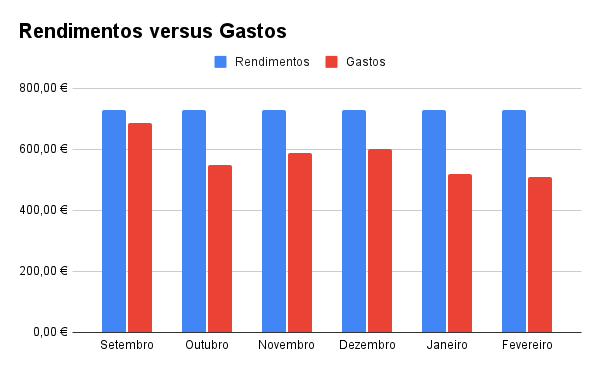
\includegraphics[width=10cm]{./rendimentos_gastos_grafico_barra.png}
					\caption{Rendimentos vs Gastos}\label{fig:barra}
					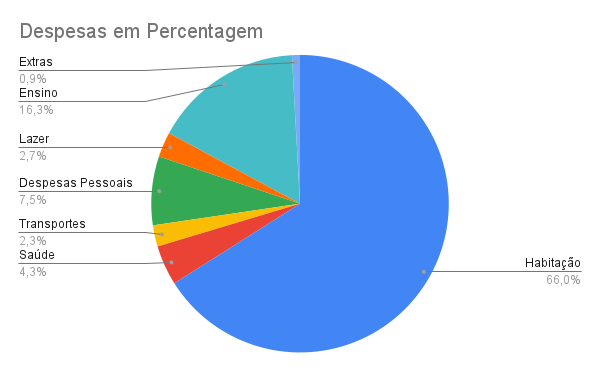
\includegraphics[width=10cm]{./despesas_percentagem.png}
					\caption{Despesas percentagem}\label{fig:circular}
				\end{center}
			\end{figure}
			
		\end{center}


		\chapter{Conclusão}
		\begin{minipage}{\textwidth}
			\hspace{1cm} Por meio deste caso de estudo, conseguimos visualizar na tabela de planejamento ~\ref{tab:planeamento } a projecção dos \
			gastos e rendimentos do estudante do mês de Setembro ao mês de Fevereiro. O total resumido do que foi ganho e \
			o que foi gasto respectivamente em cada um dos custos típicos das despesas pessoais de um indivíduo é \
			representado pela tabela de contas ~\ref{tab:contas}. 
			A proporção das suas despesas com os seus ganhos por meio do gráfico Rendimentos vs Gastos~\ref{fig:barra}.
		\end{minipage}
		\begin{minipage}{\textwidth}
			\hspace{1cm} O gráfico circular ~\ref{fig:circular} representa as despesas pessoais em percentagem, conseguimos notas que mais de \
			80\% das despesas são relacionadas à habitação e ensino. Custo esse extremamente lógico, se contextualizarmos \
			com o estágio atual da sua vida.
		\end{minipage}
		\begin{minipage}{\textwidth}
			\hspace{1cm} O planejamento das finanças pessoais é sempre uma projecção, e cabe ao indivíduo segui-lo ou não.
			\vskip 0.01cm
		\end{minipage}
		\begin{minipage}{\textwidth}
			\hspace{1cm} Portanto, caso o estudante universitário consiga cumprir com o planejamento, terá uma vantagem econômica \
			com essa gestão das finanças pessoais. Conseguimos notar o resumo do seu saldo acumulado por meio da tabela de resumos ~\ref{fig:barra}, \
			concluímos que o mesmo consegue salvar em 6 meses até \textbf{924,80€}. Assim sendo, conseguimos provar a vantagem do \
			planeamento das finanças pessoais.
		\end{minipage}

	\begin{thebibliography}{99}

		% * A consulta bibliográfica relativa ao tema e a citação são obrigatórias.
		\bibitem{intro:intro}
			\textbf{Associação de politécnicos do norte:}
				\url{https://bibliotecadigital.ipb.pt/bitstream/10198/24948/1/Catarina%20Marinho.pdf} \\
			\textbf{Congresso de Iniciação Científica:}
				\url{https://conic-semesp.org.br/anais/files/2015/1000021289.pdf}
		\bibitem{intro:desenvolvimento}
			\textbf{Jornal de Negocios:}
				\url{https://jornaldenegocios.pt/opiniao/deans-corner/joao-pinto/detalhe/mais-um-ano-letivo-a-arrancar-e-a-literacia-financeira} \\
			\textbf{Mapfre:}
				\url{https://mapfre.com/pt-br/actualidade/economia-pt-br/impacto-educacao-financeira-economia-pais/}
		\bibitem{intro:orcamento}
			\textbf{Forbes Portugal:}
				\url{https://forbespt.com/como-fazer-um-orcamento-pessoal/}
		\bibitem{intro:citacao}
			\textbf{O'REILLY}
				\url{https://www.oreilly.com/library/view/information-literacy-in/9781843345169/xhtml/B9781843345152500111.htm}
		\bibitem{intro:bibliografia}
			\textbf{Wikipedia:} \url{https://pt.wikipedia.org/wiki/Alan_Greenspan}
	\end{thebibliography}

\end{document}

% * Image bibliography
% * https://iconscout.com/illustration/finance-calculator-6771660
% * Quotes list
% * https://www.chime.com/blog/15-quotes-from-our-favorite-money-saving-experts/
% * https://www.brainyquote.com/quotes/john_w_rogers_jr_624550

